\documentclass[titlepage]{article}
\usepackage[left=15mm,right=15mm,top=1in,bottom=1in]{geometry}
\usepackage{framed}
\usepackage{caption}
\usepackage{amsmath}
\usepackage{imakeidx}
\usepackage{graphicx}
\usepackage{array}

\newcolumntype{C}[1]{>{\centering\arraybackslash} m{#1cm}}
\graphicspath{{./img/}}

\makeindex

\title{Autonomous Pool Playing Robot\\~\\High-Level Architectural Design}
\author{
	Ernest Selman\\selmae@mcmaster.ca\\1201291\\~\\\and
	Guy Meyer\\meyerg@mcmaster.ca\\1320231\\~\\\and
	Eric Le Fort\\leforte@mcmaster.ca\\1308609\\~\\\and
	Andrew Danha\\danhaas@mcmaster.ca\\1223881\\~\\\and
	Derek Savery\\saverydj@mcmaster.ca\\1219142\\~\\
}
 
\begin{document}
\maketitle
\tableofcontents
\newpage
\listoftables
\listoffigures


\vfill
\begin{table}[!htbp]
\centering
\begin{tabular}{| C{3} | C{2} | C{5} | C{2.5} |}\hline
	Date			&Revision \#	&Comments					&Authors\\\hline
	6/12/2016		&1				&- Document initialized		&Eric Le Fort\\\hline
	7/12/2016		&1				&- First draft completion	&Guy Meyer\newline Ernest Selman\newline Derek Savery\newline Andrew Danha\newline Eric Le Fort\\\hline
\end{tabular}
\caption{Revision History}
\end{table}
\newpage
\section{Introduction}
This document will describe the high-level hardware architecture of the Autonomous Pool Playing Robot. This document is intended to prepare the hardware team for implementation of each component discussed within.
\subsection{System Description}
The hardware part of this system will consist of the mechanical, electromechanical, and electrical components which in combination will form the autonomous pool playing robot.\\\\
The mechanical components will form the structure of the robot in order to allow the end effector to move in the X, Y, and Z axis, rotate about the Z axis, and provide the support to maintain the stability of the system. The electromechanical components will facilitate motion of the robot including actuating the end-effector. The electrical components will power the entire system as well as deliver signals to the electromechanical devices in order to drive the motion of the robot.
\subsection{Overview}
This document has three sections not including this one. The first section is dedicated to the mechanical components, the second section is dedicated to the electromechanical components, and the third section is dedicated to the electrical components.\\\\
For each mechanical component there is a subsection containing a diagram of that component, a subsection dedicated to the description of that component, and a subsection dedicated to the requirements of that component.\\\\
For each electro-mechanical component there is a subsection dedicated to the description of that component and a subsection dedicated to requirements of that component.\\\\
The electrical section begins with a subsection containing a context diagram to illustrate the interactions between components. For each electrical component there is a subsection dedicated to the description of that component, a subsection dedicated to the requirements of that component, and a subsection dedicated to any monitored and controlled variables for that component.

\subsection{Naming Conventions \& Definitions}
This section outlines the various definitions, acronyms and abbreviations that will be used throughout this document in order to familiarize the reader prior to reading.
\newpage
\subsubsection{Definitions}
Table \ref{tab:Definitions} lists the definitions used in this document. The definitions given below are specific to this document and may not be identical to definitions of these terms in common use. The purpose of this section is to assist the user in understanding the requirements for the system.
\begin{table}[h!]
\centering
\caption{Definitions}
\begin{tabular}{| C{6} | p{6cm} |}\hline
	\textbf{Term}	&\textbf{\centering Meaning}\\\hline
	X-axis					&Distance along the length of the pool table\\\hline
	Y-axis					&Distance across the width of the pool table\\\hline
	Z-axis					&Height above the pool table\\\hline
	End-effector			&The end of the arm that will strike the cue ball\\\hline
	$\theta$				&Rotational angle of the end-effector\\\hline
	Cue 					&End-effector\\\hline
	Personal Computer		&A laptop that will be used to run the more involved computational tasks such as visual recognition and the shot selection algorithm\\\hline
	Camera					&Some form of image capture device (e.g. a digital camera, smartphone with a camera, etc.)\\\hline
	Table State				&The current positions of all the balls on the table\\\hline
	Entity					&Classes that have a state, behaviour and identity (e.g. Book, Car, Person, etc.)\\\hline
	Boundary				&Classes that interact with users or external systems\\\hline
\end{tabular}
\label{tab:Definitions}
\end{table}

\subsubsection{Acronyms \& Abbreviations}
Table \ref{tab:Acronyms} lists the acronyms and abbreviations used in this document.
\begin{table}[h!]
\centering
\caption{Acronyms and Abbreviations}
\begin{tabular}{| p{6cm} | p{6cm} |}\hline
	\textbf{Acronym/Abbreviation}	&\textbf{Meaning}\\\hline
	VR								&Visual Recognition\\\hline
	PC								&Personal Computer\\\hline
	$\mu$C							&Micro-Controller\\\hline
	EE								&End-Effector\\\hline
	EEB								&End-Effector Base\\\hline
	EEA								&End-Effector Arm\\\hline
	PWM								&Pulse Width Modulation\\\hline
	I/O								&Input/Output\\\hline
\end{tabular}
\label{tab:Acronyms}
\end{table}



\newpage
\section{Mechanical System}
This section will go into further detail regarding each mechanical component that is to be designed as part of this system.
\subsection{X-Rails}
\textbf{Description}\\
The X-rails are the largest source of translational motion in the system. They are responsible for carrying the rest of the system along the length of the table. The motion will be induced by two motors that apply power from the end of this axis. Both sides of the table will be equipped with an X-rail since it will carry most of the load and that will provide greater stability in an evenly distributed manner.\\\\
\textbf{Requirements}\\
The X-rails will be required to run the full length of the pool table. Furthermore, they will be required to support the full weight of the rest of the mechanical components by transferring it to the sides of the pool table.
\begin{center}
	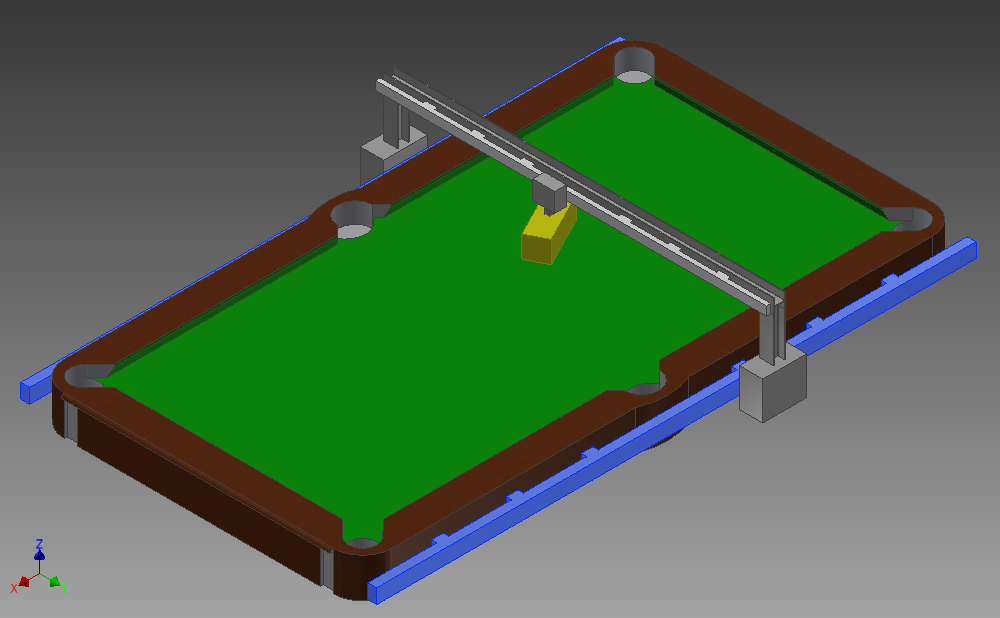
\includegraphics[width = 0.9\textwidth]{xRails1.png}
\captionof{figure}{X-Rails relative to the table (found in blue) }
\label{fig:xRailFig}
\end{center}

\newpage
\subsection{Y-Rails}
\textbf{Description}\\
The Y-rail allows for translational motion of the end effector along the width of the table. The support for this component will be provided by the bridge. Although if the rails are strong enough on their own the bridge is not needed and the rails will connect to the arms themselves.\\\\
\textbf{Requirements}\\
The purpose of the Y-rail is to provide motion of the end-effector base in the Y-axis with low friction. It must allow traversal of the entire width of the table smoothly. It is not a requirement to support the EE since that will be done by the bridge, although these components may become one if the Y-rail is strong enough on its own.
\begin{center}
	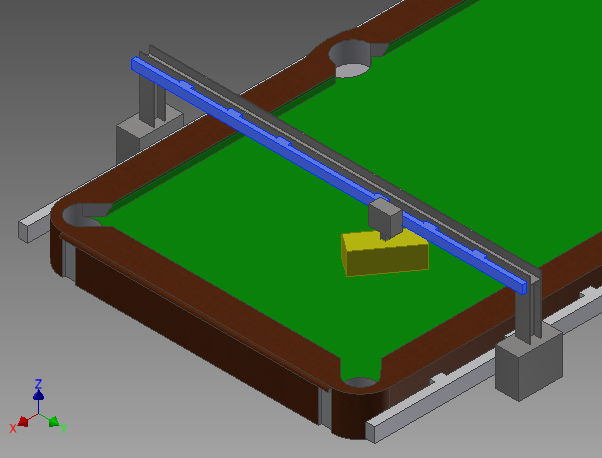
\includegraphics[width = 0.9\textwidth]{yRail1.png}
\captionof{figure}{Y Rail relative to the table (found in blue) }
\label{fig:yRailFig}
\end{center}

\newpage
\subsection{Camera Mount}
\textbf{Description}\\
The camera mount is the component that holds the device responsible for image capture to be used by the VR. The structure of the mount may either be a bridge that runs across the width of the table (y-axis) and over the arms or a crane-like structure that extends from one side to the center of the table. The design of the camera mount may also include a lamp to supplement the lighting for optimal pictures.\\\\
\textbf{Requirements}\\
The camera mount is required to ensure that the mobile device is located sufficiently high and parallel to the table. This is to allow the VR software to be able to consistently analyze the image properly. It is vital that the structure does not interfere with any of the moving mechanical components present. Furthermore, it will be designed in order to minimize the amount it gets in the user's way while they take their shot. The robot may sometimes interfere with getting an unobstructed view of the table. Therefore, the robot may be required to move out of the way for the image capture process.
\begin{center}
	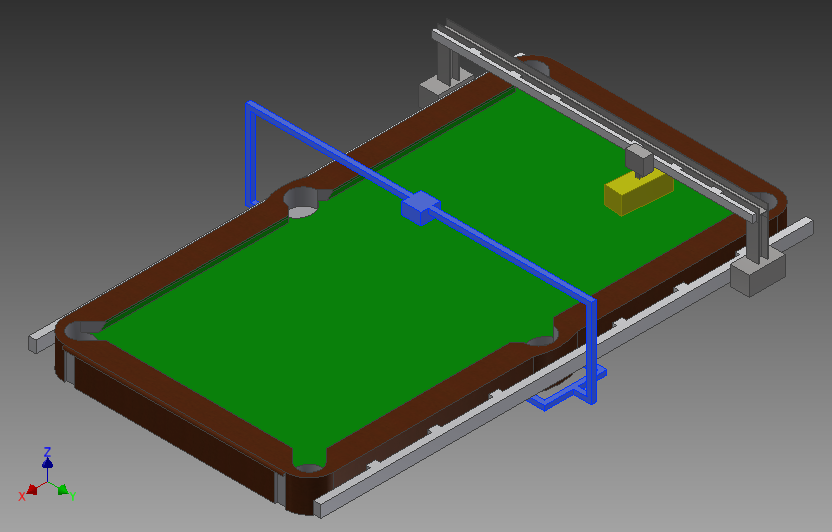
\includegraphics[width = 0.9\textwidth]{cameraMountYAxis.png}
\captionof{figure}{Camera Mount relative to the table (found in blue) }
\label{fig:cameraMount}
\end{center}

\newpage
\subsection{Arm}
\textbf{Description}\\
Extruding vertically from the arm base, the arm connects to the Y-rail and provides stability between the two axes of motion. The arm moves as one with the arm base since they both provide support for the bridge.\\\\
\textbf{Requirements}\\
The arm will be required to remain rigidly perpendicular to the X-rail while supporting its weight (i.e. remain upright without buckling). It is also required to maintain stability when faced with disturbances originating from the end-effector.
\begin{center}
	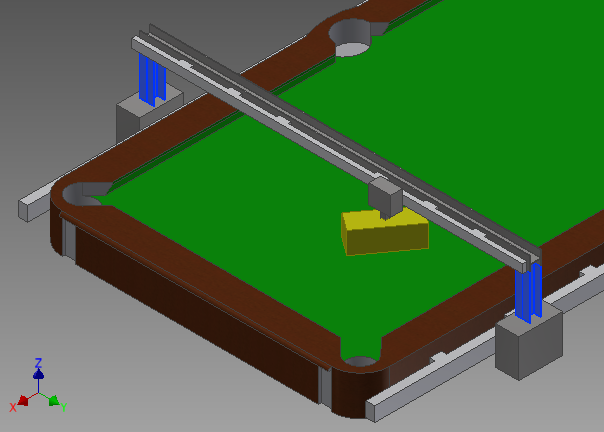
\includegraphics[width = 0.9\textwidth]{arms.png}
\captionof{figure}{Arms relative to the table (found in blue)}
\label{fig:armFig}
\end{center}

\newpage
\subsection{Arm Base}
\textbf{Description}\\
The arm base is a connection between the X-rail and the arm. The arm base is a sturdy component that will move in the X-direction. There are two arm bases, one on each X-rail.\\\\
\textbf{Requirements}\\
The arm base will be required to move the full length of the X-rail with small amounts of friction. Furthermore, the arm base will be required to support the arm while keeping the arm in a vertical position.
\begin{center}
	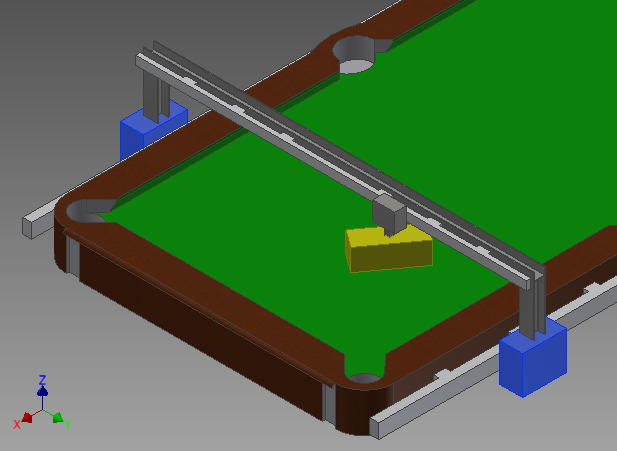
\includegraphics[width = 0.9\textwidth]{armBase.png}
\captionof{figure}{Arm Base relative to the table (found in blue)}
\label{fig:armBaseFig}
\end{center}

\newpage
\subsection{Bridge}
\textbf{Description}\\
The bridge provides support for the Y-rail. The bridge component will be unnecessary if the Y-rail provides enough support by itself. If that is not the case, the bridge will increase support along the entirety of the system's motion in the Y-direction. The bridge will connect to the arms on both sides of the table.\\\\
\textbf{Requirements}\\
The bridge will be required to remain parallel with the widthwise edge of the pool table. Furthermore, the bridge will be required to both provide support such that the Y-rail does not bend and transfer the weight of the end-effector components to the arms.
\begin{center}
	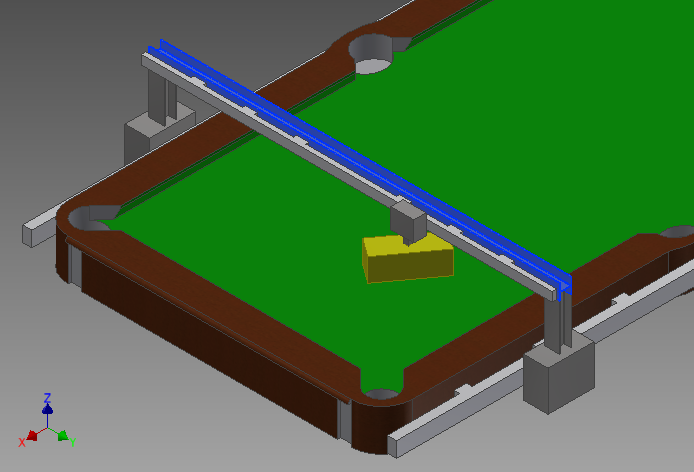
\includegraphics[width = 0.9\textwidth]{bridge.png}
\captionof{figure}{Bridge relative to the table (found in blue)}
\label{fig:bridgeFig}
\end{center}

\newpage
\subsection{End-Effector}
\textbf{Description}\\
The EE is used to strike the cue ball that is resting on the table. The EE will have rotational capabilities either on its own or along with the EEA.\\\\
\textbf{Requirements}\\
The EE will be required to accurately provide an impulsive force to the cue ball. Its electromechanical/pneumatic characteristics are further described in the Electromechanical Systems section.
\begin{center}
	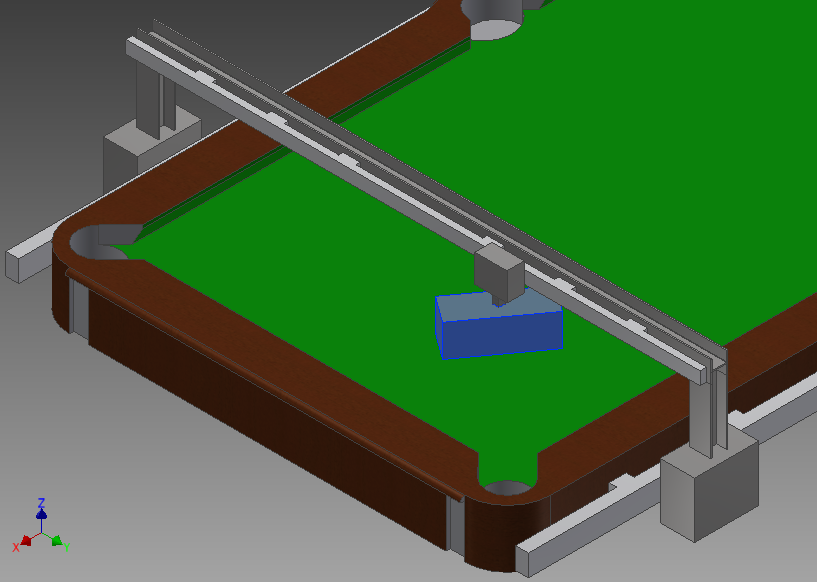
\includegraphics[width = 0.9\textwidth]{endEffector.png}
\captionof{figure}{End-Effector relative to the table (found in blue)}
\label{fig:eeFig}
\end{center}

\newpage
\subsection{End-Effector Arm}
\textbf{Description}\\
The End-Effector Arm (EEA) is the connector between the EEB and the EE. It could be a shaft from the motor or a solid piece that is static relative to the EE but rotates in relation to the EEB. The purpose of this component is to lower the height of the EE while providing stability from the Y-rail.\\\\
\textbf{Requirements}\\
The EEA will be required to remain perpendicular to the surface of the pool table. Furthermore, the EEA will be required to transfer torque to the EE and support the weight of the EE.
\begin{center}
	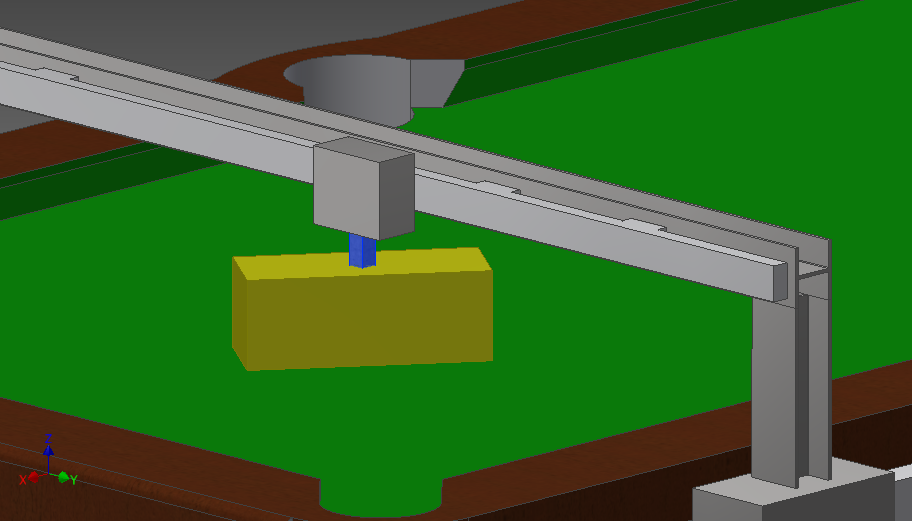
\includegraphics[width = 0.9\textwidth]{efArm.png}
\captionof{figure}{End-Effector Arm relative to the table (found in blue)}
\label{fig:eeaFig}
\end{center}

\newpage
\subsection{End-Effector Base}
\textbf{Description}\\
The End-Effector Base (EEB) supports the EEA and connects it to the Y-rail. It is the connection between the motion of the Y-rail and the EEA. The EEB will likely connect to a belt attached to a motor. It also contains the actuator that provides rotation to the EE through the EEA.\\\\
\textbf{Requirements}\\
The EEB will be required to move the full length of the Y-rail with a small amount of friction between the Y-rail and itself. Furthermore, the EEB will be required to affix the EEA to the Y-rail. It must also be able to rotate the EEA in order to change the direction of the EE.
\begin{center}
	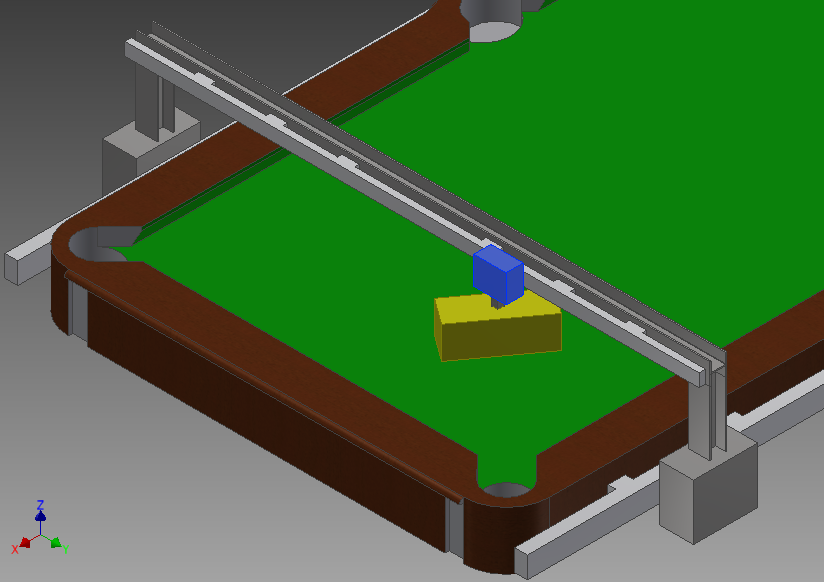
\includegraphics[width = 0.9\textwidth]{efBase.png}
\captionof{figure}{End-Effector Base relative to the table (found in blue)}
\label{fig:eebFig}
\end{center}


\newpage
\section{Electromechanical System}
This section will go into further detail regarding each electromechanical component that is to be designed as part of this system.
\subsection{X-Rail Motors}
\textbf{Description}\\
As mentioned above, the X rails will traverse the length of the table proving motion in the x-axis. In order to generate this motion, sufficiently strong motors are required to provide power in each direction. There will be two motors due to the width of the table. Both will act synchronously in order to provide equal motion on both sides. The motors will be stepper motors which will allow for accurate measurements of linear distance found through the counting of steps. The motion of the motor will be tranlated onto the Arm Base through the use of belts or rotational (worm) gears. This allows the motors to remain in one place while the mechanical structure is sliding back and forth (identical belts will be included on both sides). The motors will also be geared in order increase precision and vary the torque applied on the motor.\\\\
\textbf{Requirements}\\
Based on the specifications of the components moved by the X-rail motor (physical mass, friction, and size of the system) the motor's requirements will be determined. It is imperative that the motor will have enough power to drive the motion. The motor is also required to have a sufficient number of steps in order to track the motion and will be geared accordingly to achieve proper accuracy. Both motors will have the same specifications which will maintain symmetry. 

\subsection{Y-Rail Motor}
\textbf{Description}\\
The Y-rail motor will power the movement required in the Y-direction. Only one motor is needed since the affected components will be supported at a single point on the Y-rail. Similar to the X-rail motors, a stepper motor will be used in order to keep track of the distance traveled along the rail. This motor will be geared as well which will result in a higher resolution of steps and reduce the torque applied on the motor. Additionally, belts will be used in this application as well (similar to the X-Rail Motors) where either a belt or a rotational (worm) gear will be used to translate the rotational motion of the rail gears onto a linear motion in the axis of the y axis.\\\\
\textbf{Requirements}\\
The electromechanical specifications are reliant on the physical properties of the affected system such as friction coefficients, mass, and size of the components. The motor is also required to have a sufficient number of steps but will be geared if found to require higher accuracy. Finally the motor is required to connect to the motion of the rail either through a belt or another means.

\subsection{Rotational Motor}
\textbf{Description}\\
The Rotational Motor is responsible for properly orienting the EE in the proper direction. It will spin about the axis of the EEA which is attached to the EE at its bottom end. The rotational motor will be housed in the EEB since it provides the most support for a high torque motor. Furthermore, the shaft of the motor will be pointing straight down towards the table to allow the attached EE to reach as close to the table as possible without ball interference. Once the proper orientation is achieved it must remain firmly in place to allow the EE to maintain accuracy whilst attempting a shot. The use of steps or another feedback mechanism will track the current angle of the EE.\\\\
\textbf{Requirements}\\
The motor is required to spin at least 360 degrees in order to cover all the possible shot angles. The positioning must have a high enough accuracy such that an orientation is achieved within acceptable error. As briefly mentioned in the description section above, the motor must also resist disturbances from the EE to avoid loss of accuracy. Although a stepper motor would be preferred any motor with the ability to track rotational displacement may be used.

\subsection{End-Effector Actuator}
\textbf{Description}\\
The End-Effector (EE) is responsible for striking the cue ball in order to play the game. It is not yet decided whether the actuator will be pneumatic or electromechanical, but either way the final translation of energy to the ball is similar. If pneumatic actuators are chosen then electrical valves will be used to control the flow of air into the pneumatic chamber.\\\\
\textbf{Requirements}\\
It is very important that the actuator applies sufficient power to the ball so that it can score from all feasible positions on the table. Additionally, in order to direct itself onto the proper orientation it is required to rotate a full 360 degrees. The accuracy of this motion is key to ensuring a proper shot and must be tracked in order to maintain repeatability. The EE must also be easy to maneuver since it is moved by other motors and supported by other structures. Finally, the EE must not interfere with the game/balls in any way, after striking the balls it must allow the balls to roll freely. This works conjointly with the fact that it should take up the least amount of space as possible to increase its workspace.



\section{Electrical System}
This section will go into further detail regarding each electrical component that is to be designed as part of this system.
\subsection{Context Diagram}
The following diagram is intended to illustrate the interactions between the electrical components in this system.
\begin{center}
	\includegraphics[width = \textwidth]{elecContextDiagram.png}
\captionof{figure}{Electrical subsystem context diagram.}
\label{fig:elecContextDiagramFig}
\end{center}

\subsection{Power Supply}
\textbf{Description}\\
The power supply is the source of power for the entire system.\\\\
\textbf{Requirements}\\
A single source of power that provides enough voltage and current to be distributed to all components of the system. The power supply for this system will be a single 110 AC V standard outlet.\\\\
\textbf{Monitored \& Controlled Variables}\\
None.

\newpage
\subsection{Transformer}
\textbf{Description}\\
A transformer is an electrical device that transforms the input voltage to a desired output voltage through electromagnetic induction.\\\\
\textbf{Requirements}\\
The system will require a certain level of voltage, most likely less than 110 AC V. This device will regulate the voltage to the level required by the system in order to avoid damaging the system and ensure the safety of users.\\\\
\textbf{Monitored \& Controlled Variables}\\
The input voltage of the transformer will be 110 AC V from the standard outlet. The transformer will then reduce this voltage to the prescribed level for the system.

\subsection{AC to DC Converter}
\textbf{Description}\\
This device converts an input AC voltage to an equivalent DC voltage.\\\\
\textbf{Requirements}\\
All components of the system will operate on DC voltage. This device must be able to convert the AC voltage that it receives from the transformer into DC voltage to be delivered to the system.\\\\
\textbf{Monitored \& Controlled Variables}\\
None.

\subsection{$\mu$C}
\textbf{Description}\\
A small computer with programmable Input/Output (I/O) peripherals that will govern the operation of the machine by generating the appropriate signals as computed.\\\\
\textbf{Requirements}\\
Since the $\mu$C will receive instructions from the PC via wireless protocol, a bluetooth or a WiFi module will be required. The $\mu$C must also have enough I/O ports for the peripherals (such as sensors and actuators).\\\\
\textbf{Monitored \& Controlled Variables}\\
The $\mu$C?s required power supply depends on the model chosen for the system. The $\mu$C will output control signals (HIGH or LOW) to the controllers and will implement PWM in order to operate the actuators at the desired level of power. The $\mu$C may also power the sensors used by the system. A simple circuit or voltage regulator will be used to regulate the voltage level from the $\mu$C to the sensor. The sensors will send back analog or digital signals to the $\mu$C which it will then read and interpret accordingly.

\subsection{Controllers}
\textbf{Description}\\
These devices are an intermediary between the $\mu$C/power supply and the actuators. The controllers will govern the performance of the actuators.\\\\
\textbf{Requirements}\\
The controllers must be able to operate under the required voltages of their respective actuators.\\\\
\textbf{Monitored \& Controlled Variables}\\
They will receive appropriate power from the power supply and control signals (HIGH or LOW) from the $\mu$C. The control signals it receives from the $\mu$C will power the actuators accordingly.

\newpage
\subsection{Actuators}
\textbf{Description}\\
The actuators will be responsible for generating all motion within the system. They will consist of two motors responsible for moving the end-effector along the length of the table, one motor for moving along the width, one motor for rotating the end-effector, and an actuator responsible for the shooting motion of the end-effector.\\\\
\textbf{Requirements}\\
The motors must provide ample torque to move the system?s components along/about the axis of the system. The end-effector actuator must output enough force and momentum to shoot the cue-ball fast enough across the table as well as be able to adjust the amount of force appropriately.\\\\
\noindent\textbf{Monitored \& Controlled Variables}\\
All actuators in the system will receive power from their respective controllers. The actuators? output (in terms of force/torque) is reliant on the power received from the controllers.

\subsection{Sensors}
\textbf{Description}\\
Sensors will aid in verifying the system?s current position and orientation.\\\\
\textbf{Requirements}\\
The sensors used in the system must operate in accordance with the $\mu$C. The $\mu$C will be required to read the analog/digital signals outputted by the sensor therefore this output voltage must be within the $\mu$C?s range of acceptable input voltages.\\\\
\textbf{Monitored \& Controlled Variables}\\
They may receive power from the $\mu$C and relay analog or digital signals (depending on the type of sensor) back to the $\mu$C.

\end{document}



